\documentclass[
11pt, % The default document font size, options: 10pt, 11pt, 12pt
codirector, % Uncomment to add a codirector to the title page
]{charter} 

% El títulos de la memoria, se usa en la carátula y se puede usar el cualquier lugar del documento con el comando \ttitle
\titulo{Título del proyecto} 

% Nombre del posgrado, se usa en la carátula y se puede usar el cualquier lugar del documento con el comando \degreename
\posgrado{Carrera de Especialización en Sistemas Embebidos} 
%\posgrado{Carrera de Especialización en Internet de las Cosas} 
%\posgrado{Carrera de Especialización en Intelegencia Artificial}
%\posgrado{Maestría en Sistemas Embebidos} 
%\posgrado{Maestría en Internet de las cosas}

% Tu nombre, se puede usar el cualquier lugar del documento con el comando \authorname
\autor{SISE-AS versión A} 

% El nombre del director y co-director, se puede usar el cualquier lugar del documento con el comando \supname y \cosupname y \pertesupname y \pertecosupname
\director{Nombre del Director}
\pertenenciaDirector{pertenencia} 
% FIXME:NO IMPLEMENTADO EL CODIRECTOR ni su pertenencia
\codirector{John Doe} % para que aparezca en la portada se debe descomentar la opción codirector en el documentclass
\pertenenciaCoDirector{FIUBA}

% Nombre del cliente, quien va a aprobar los resultados del proyecto, se puede usar con el comando \clientename y \empclientename
\cliente{Nombre del cliente}
\empresaCliente{Empresa del cliente}

% Nombre y pertenencia de los jurados, se pueden usar el cualquier lugar del documento con el comando \jurunoname, \jurdosname y \jurtresname y \perteunoname, \pertedosname y \pertetresname.
\juradoUno{Nombre y Apellido (1)}
\pertenenciaJurUno{pertenencia (1)} 
\juradoDos{Nombre y Apellido (2)}
\pertenenciaJurDos{pertenencia (2)}
\juradoTres{Nombre y Apellido (3)}
\pertenenciaJurTres{pertenencia (3)}
 
\fechaINICIO{30 de abril de 2021}		%Fecha de inicio de la cursada de GdP \fechaInicioName
\fechaFINALPlan{18 de junio de 2021} 	%Fecha de final de cursada de GdP
\fechaFINALTrabajo{15 de mayo de 2022}	%Fecha de defensa pública del trabajo final

\def\codigo{SISE-RS}
\newcommand{\req}[1]{\textbf{[\codigo-#1]:}}

\begin{document}

\maketitle
\thispagestyle{empty}
\pagebreak


\thispagestyle{empty}
{\setlength{\parskip}{0pt}
\tableofcontents{}
}
\pagebreak


\section*{Registros de cambios}
\label{sec:registro}

\begin{table}[ht]
\label{tab:registro}
\centering
\begin{tabularx}{\linewidth}{@{}|c|X|c|@{}}
\hline
\rowcolor[HTML]{C0C0C0} 
Revisión & \multicolumn{1}{c|}{\cellcolor[HTML]{C0C0C0}Detalles de los cambios realizados} & Fecha      \\ \hline
A & Creación del documento & 11/08/2021 \\ \hline
\end{tabularx}
\end{table}

\pagebreak

\section{1. Introducción}
\label{sec:introduccion}

\subsection{Propósito}
\label{sub:proposito}

Este documento representa una especificación de requerimientos de software para un \emph{Evaluador de microcontroladores para misiones espaciales}.
El documento está dirigido a las personas que trabajen en la esfera de: análisis, diseño, implementación o pruebas.

\subsection{Ámbito del sistema}
\label{sub:ambito}

El nombre del sistema será SISE y permitirá evaluar si el microcontrolador deseado puede tener un uso espacial.
Además, facilitará la valoración de las técnicas de mitigación de errores.
El proyecto incluirá dos módulos que funcionarán en ámbitos distintos.
Ellos serán:

\begin{itemize}
	\item Inyector por consola de comando (CCI)
	\item Proceso de dispositivo bajo prueba (DUT)
\end{itemize}

El ámbito de CCI será el ordenador del usuario; mientras que el proceso de DUT funcionará en el microcontrolador.

\subsection{Definiciones, acrónimos y abreviaturas}
\label{sub:definiciones}

\begin{enumerate}
	\item Definiciones:
		\begin{itemize}
			\item Single event effect: efecto de una partícula enérgicamente cargada sobre un microcontrolador.
			\item Single event funtional interrupt: interrupción causada por el impacto de una sola partícula que conduce a una no funcionalidad temporal.
			\item Single event upset: pulso transitorio en la lógica o circuitos de apoyo. Son \emph{soft-errors} no destructivos.
			\item Soft-error: tipo de error en donde una señal o dato es incorrecto.
		\end{itemize}
	\item Acrónimos:
		\begin{itemize}
			\item API: interfaz de programación de aplicaciones.
			\item DUT: dispositivo bajo prueba (microcontrolador).
			\item FOM: figura de mérito.
			\item IEEE: Instituto de Ingenieros Eléctricos y Electrónicos.
			\item OCD: on-chip debugger.
			\item SEE: single event effect.
			\item SEFI: single event functional interrupt.
			\item SEU: single event upset.
			\item TBD: a ser determinado.
			\item UART: universal asynchronous receiver-trasmitter.
		\end{itemize}
	\item Abreviaturas:
		\begin{itemize}
			\item Std: estándar.
		\end{itemize}
\end{enumerate}

\subsection{Referencias}
\label{sub:referencias}
INVAP - Propuesta de tesis: sistema de inyección de soft-errors.

\subsection{Visión general del documento}
\label{sub:vision}

Este documento se realizó según lo especificado en el estándar IEEE Std. 830-1998.

\section{2. Descripción general}
\label{seb:descripcion}

\subsection{Perspectiva del producto}
\label{sub:perspectiva}

El proyecto aquí especificado es independiente de otros sistemas y no tiene relación con otros productos.
Como se especificó en subsección \ref{sub:proposito}, se realizarán los siguientes módulos: CCI y Proceso de DUT.

El módulo CCI tendrá la función de generar SEFIs que introduzcan SEUs.
Los SEFI-SEU serán inyectados de forma electrónica; esto simulará los efectos de una partícula cargada que impacta en el DUT.
Como se explicó en la subsección \ref{sub:ambito}, el módulo residirá en el ordenador del usuario.
La interacción se realizará a través de una \emph{consola de línea de comandos}.
Finalmente, se podrá configurar el ensayo a realizar.

En la figura \ref{fig:CCIbloques} se puede observar el diagrama en bloques del módulo CCI.
La consola de usuario será la interfaz que el ingeniero utilice para usar el sistema.
El controlador de ensayos procesará los datos ingresados por el usuario, coordinará los SEFI-SEU y observará los reportes del DUT.
El servidor OCD se encargará de realizar lecturas de registros y las inyecciones de SEFI-SEU.
El OCD API será la interfaz entre el Controlador de ensayos y el Servidor OCD; utilizará un protocolo TBD.
La Interfaz serie capturará los informes del DUT.
Finalmente, la Persistencia de datos almacenará toda la información generada durante la ejecución del ensayo.

\begin{figure}[h!]
	\centering
	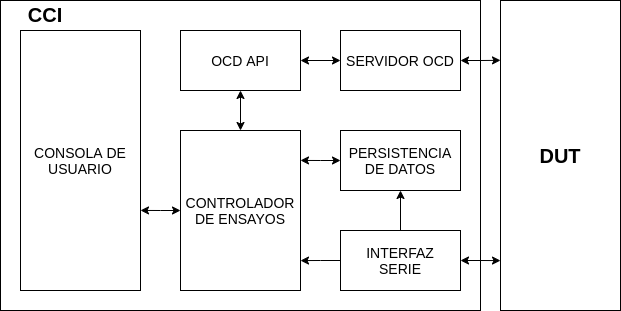
\includegraphics[width=\textwidth]{./Figuras/CCIbloques.png}
	\caption{Diagrama en bloques del módulo CCI.}
	\label{fig:CCIbloques}
\end{figure}

En la figura \ref{fig:DUTbloques} se puede observar el diagrama en bloques del módulo \emph{Proceso de DUT}.
El firmware deberá recorrer todos los periféricos del DUT.
En cada periférico se generará una operación de autovalidación.
Finalizada la verificación de todos los periféricos, el firmware enviará un reporte a través de la UART.
Finalmente, el bloque de debugger será el punto de ingreso para las SEFI-SEU.

\begin{figure}[h!]
	\centering
	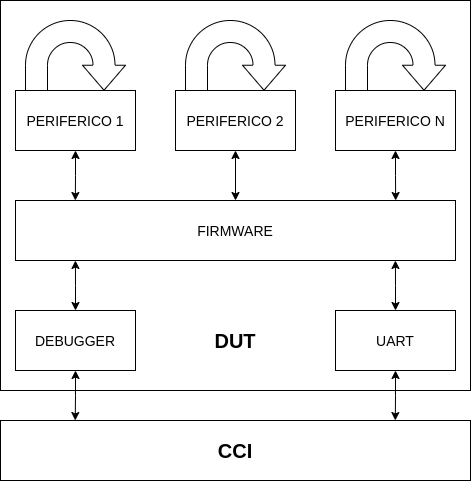
\includegraphics[width=0.7\textwidth]{./Figuras/DUTbloques.png}
	\caption{Diagrama en bloques del módulo Proceso de DUT.}
	\label{fig:DUTbloques}
\end{figure}

\subsection{Funciones del producto}
\label{sub:funcionesProducto}

El software aquí especificado brindará las siguientes funcionalidades:

\begin{enumerate}
	\item Referentes al CCI:
		\begin{enumerate}
			\item Generará de una interfaz de usuario.
			\item Permitirá configurar el ensayo a realizar.
			\item Activará el Proceso de DUT.
			\item Observará la salida del DUT.
			\item Inyectará SEFI-SEU en el DUT.
			\item Persistirá las operaciones, entradas y salidas.
			\item Generará informes del ensayo realizado.
		\end{enumerate}
	\item Referentes al Proceso de DUT:
		\begin{enumerate}
			\item Verificará el estado de los periféricos del DUT.
			\item Detectará si el DUT perdió su secuencia.
			\item Generará reportes de estado de periféricos y secuencia.
			\item Permitirá que CCI configure el alcance de la secuencia.
			\item Permitirá que CCI maneje el flujo de su secuencia.
		\end{enumerate}
\end{enumerate}

\subsection{Características de los usuarios}
\label{sub:usuarios}

Los usuarios finales de este producto son ingenieros de desarrollo de INVAP.

\subsection{Restricciones}
\label{sub:restricciones}

Las restricciones del desarrollo del sistema son las siguientes:

\begin{itemize}
	\item Utilización de repositorio con control de versiones \emph{Gitlab}.
	\item Documentación del código con \emph{Doxygen}.
	\item Utilización exclusiva del lenguaje de programación \emph{Python 3}.
\end{itemize}

\subsection{Suposiciones y dependencias}
\label{sub:suposiciones}

La suposición principal es que se tendrá acceso irrestricto al DUT seleccionado antes del día 01/01/2022.

\section{3. Arquitectura}
\label{sec:arq}

\subsection{Patrones}
\label{sub:pat}

Para este sistema se emplearan los siguientes patrones arquitectónicos:

\begin{enumerate}
	\item Inyector por consola de comando:
		\begin{enumerate}
			\item Observar y reaccionar.
			\item Segmentación de proceso.
		\end{enumerate}
	\item Proceso en DUT:
		\begin{enumerate}
			\item Observar y reaccionar.
			\item \emph{Hardware Abstraction Layer} (HAL).
		\end{enumerate}
\end{enumerate}

\subsubsection{Observar y reaccionar}
\begin{enumerate}
	\item Este patrón se utiliza cuando un conjunto de sensores se monitorean y despliegan de manera rutinaria.
	\item Uso en Inyector por consola de comando:
		\begin{enumerate}
			\item Monitoreo de reportes del DUT.
			\item Captura de eventos en la interfaz de usuario.
			\item Persistencia en memoria y generación de informes.
		\end{enumerate}
	\item Uso en Proceso en DUT:
		\begin{enumerate}
			\item Monitoreo del estado de los periféricos.
			\item Captura de inyecciones de SEFI-SEU.
			\item Reportes del estado de la secuencia.
		\end{enumerate}
\end{enumerate}


\subsubsection{Segmentación de proceso}
\begin{enumerate}
	\item Este patrón se usa al transformarse datos de una representación a otra antes de que puedan procesarse.
	\item El Inyector por consola de comando deberá transformar las salidas del DUT obtenidas entre secuencias para alimentar el proceso de generación de informes.
\end{enumerate}

\subsubsection{Hardware Abstraction Layer}
\begin{enumerate}
	\item Este patrón se utiliza para aprovechar la \emph{base de conocimiento} existente sobre una arquitectura de microcontrolador y cuando se necesita crear código que satisfaga una interfaz de programación definida.
	\item El Proceso en DUT correrá sobre un \emph{Sistema Operativo de Tiempo Real} (RTOS) definido por INVAP.
\end{enumerate}

\section{4. Diseño detallado}
\label{sec:det}

En esta sección se incluye el diseño detallado de los componentes de software.

\subsection{Inyector por consola de comando}

\begin{enumerate}
	\item Consola de usuario:
	\item Controlador de ensayos:
	\item Persistencia de datos:
	\item Interfaz serie:
	\item Servidor OCD:
	\item OCD API:
\end{enumerate}

\subsection{Proceso en DUT}

\begin{enumerate}
	\item Autovalidación de periféricos:
	\item UART:
	\item Secuencia general:
\end{enumerate}

\end{document}
